\documentclass[11pt]{article}
\usepackage[ngerman]{babel}
\usepackage{amsmath}
\usepackage{graphicx}

\title{WP Certified Tester WiSe 19 - Aufgabenblatt 5\\ \Huge{Review}}
\author{\textit{Protokollf\"uhrer:} Adrian Helberg}
\date{07.01.2020}

\begin{document}
    \maketitle
    \tableofcontents
    \newpage

    \section{Grundlegende Vorbereitung}
    \subsection{\"Anderbarkeit}
    \textbf{Pr\"ufen der Eigenschaften "`\"Anderbarkeit"'}\\~\\
    \underline{Fragestellung:}\\ \textit{"`Wie leicht macht der Code es anderen Programmierern ihn zu erweitern?"'}\\~\\
    \"Uberlegungen nach \textbf{ISO/IEC 9126}: Ermitteln des Aufwands, der zur Durchf\"uhrung vorgegebener \"Anderungen notwendig ist. \"Anderungen k\"onnen Korrekturen, Verbesserungen oder Anpassungen an \"Anderungen der Umgebung, der Anforderungen oder der funktionalen Spezifikationen einschlie\ss{}en (Analysierbarkeit, Konformit\"at, Modifizierbarkeit, Stabilit\"at, Testbarkeit).\\~\\
    In dieser Aufgabe bietet sich die Analysierbarkeit an, da das Ziel des Reviews die Analyse des Programms ist. Also der Aufwand, um M\"angel oder Ursachen von Versagen zu diagnostizieren.
    \subsection{\"Ubertragbarkeit}
    \textbf{Pr\"ufen der Eigenschaften "`\"Ubertragbarkeit"'}\\~\\
    \underline{Fragestellung:}\\ \textit{"`Wie hoch ist der Grad an Plattformunabh\"angigkeit des Codes?"'}\\~\\
    Die Portabilit\"at eines Programmcodes kann \"uber das Verh\"altnis von \"Ubertragungsaufwand und Anpassungsaufwand zum Entwicklungsaufwand einer Neuentwicklung gesch\"atzt werden: $P=1-(\"U+A):E$
    \newpage
    \section{Organisation der Review-Sitzung}
    \subsection{Rollenverteilung}
    \underline{\"Uberlegung:} Technisches Review - Fachliche Pr\"ufung eines wesentlichen Dokumentes auf \"Ubereinstimmung mit der Spezifikation mit dem Zweck der Diskussion, Entscheidungsfindung, Fehlerfindung, L\"osung technischer Probleme\\~\\
    \begin{tabular}{l|c|c|c|c|c}
        \textbf{Name} & \textbf{Manager} & \textbf{Moderator} & \textbf{Autor} & \textbf{Gutachter} & \textbf{Protokollf\"uhrer} \\ \hline
        Christine & & X & & & \\ \hline
        Rodrigo & & & & X & \\ \hline
        Adrian & X & & & & X \\ \hline
        Gruppe Walid & & & X & & \\ \hline
    \end{tabular}
    \subsection{Rollenbeschreibung}
    Manager
    \begin{itemize}
        \item Teamzusammenstellung
        \item Analyse der Ergabnisse
        \item Nimmt nicht aktiv am Review teil
    \end{itemize}
    Moderator
    \begin{itemize}
        \item Planung, Vorbereitung
        \item Diskussionsleitung
        \item Keine eigene Meinung
    \end{itemize}
    Autor
    \begin{itemize}
        \item Verfasser des Testobjektes
        \item F\"uhrt notwendige \"Anderungen durch
    \end{itemize}
    Gutachter
    \begin{itemize}
        \item Pr\"ufung des Testobjektes nach bestimmten Kriterien
        \item Fehlerprotokollierung
        \item Hervorherben guter Teile des Testobjektes
    \end{itemize}
    Protokollf\"uhrer
    \begin{itemize}
        \item Dokumentation
    \end{itemize}

    \section{Individuelle Vorbereitung}

    \subsection{Untersuchung}
    \includegraphics{klassenkopf.PNG}\\
    Abweichung: Abk\"urzung f\"ur "`Minimal bestimmende Mehrfachbedingungs\"uberdeckung"' weicht von anderen Abk\"urzungen ab.\\
    \includegraphics{abkuerzung.PNG}\\~\\
    \includegraphics{camelcase.PNG}\\
    Abweichung: Namenskonvention nicht eingehalten (\textit{camel case})

    \subsubsection{Aufgabenblatt 4}
    \textbf{Aufgabe 1.1}: Abweichung von der Spezifikation
    \begin{itemize}
        \item Entwickeln einer \textit{Klasse} f\"ur die Darstellung von Wahrheitswerttabellen
        \item $\ldots$ Print-Methoden f\"ur einzelne Vektoren [$\ldots$]
    \end{itemize}
    \includegraphics{aufgabe_1_1.PNG}
    \newpage
    \textbf{Aufgabe 1.3}\\
    Ausgabe des Tests:
    \begin{center}
        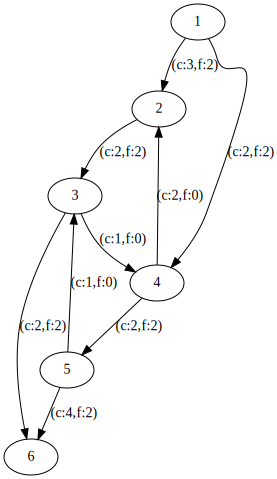
\includegraphics{result.PNG}
    \end{center}


    \subsection{Wartbarkeit}
    \underline{Wichtige Kriterien:}
    \begin{itemize}
        \item Dokumentation: Wenig Kommentare
        \item Modular: Bis auf die Implementierung einer Klasse f\"ur die Darstellung von Wahrheitstabellen, Objekt und Tests voneinander gekapselt und in einzelnen Klassen umgesetzt
        \item GOTO-Befehle: Keine Spr\"unge
        \item Verst\"andlichkeit von Anweisungen: Ausreichend gegeben
        \item Vermeiden globaler Variablen: Ausreichend gegeben
        \item Parametrisierbarkeit: Keine Skalierung auf interne Typen
        \item Assertionen: Ausreichend gegeben
        \item Umfang automatisierter Tests: Gering
        \item Verwendung von allg. bekannten Entwurfsmustern: Nein
    \end{itemize}


    \subsection{Skalierbarkeit}
    Geringe Skalierbarkeit

    \section{Durchf\"uhrung der Review-Sitzung}
    \subsection{Bewertung}
    Die Review-Sitzungen findet am 07.01.2020 statt.

    \section{Evaluation der Review-Sitzung}
    \subsection{Ergebnisse}
    Die Review-Sitzungen findet am 07.01.2020 statt.
    \subsection{Beobachtungen}
    Die Review-Sitzungen findet am 07.01.2020 statt.


\end{document}